\documentclass[compress]{beamer}
\usepackage{graphicx,amsmath,amsthm,verbatim,bm}
\usepackage{longtable}
\usepackage{booktabs}       % professional-quality tables
\usepackage{tabularx}
\usepackage{multirow}
%\usetheme{Copenhagen}
%\useoutertheme[{options}]{tree}
%\setbeamertemplate{footline}[page number]
%\useoutertheme{infolines}
%\setbeamertem plate{headlirne}{}
%\useinnertheme{circles}
\usepackage{comment}
\setbeamertemplate{footline}[frame number]
%\usepackage{times}
%\usepackage[tbtags]{amsmath}
%\usepackage{amssymb}
\usepackage{amsfonts}
\usepackage{multirow}
%\usepackage{slfortheorems}
\usepackage{epsfig}
\usepackage{graphicx}
%\usepackage[small]{caption}
\usepackage[square]{natbib}
%\newcommand{\newblock}{}
\bibpunct{(}{)}{;}{a}{}{,}
\bibliographystyle{ims}
%\usepackage[letterpaper]{geometry}
\usepackage{color}
\setlength{\parindent}{0pt}
\usepackage{bbding}
\usepackage{longtable, booktabs}
\usepackage{amsfonts}
\usepackage{lipsum}
\usepackage{tikz} 
\usetikzlibrary{arrows, snakes, backgrounds, patterns, matrix, shapes, fit, 
calc, shadows, plotmarks}
\useinnertheme{circles}
\usepackage{tabularx}

\def\spacingset#1{\renewcommand{\baselinestretch}%
  {#1}\small\normalsize} \spacingset{1}
  
  \newcommand{\dblink}{\texttt{\upshape \lowercase{d-blink}}} % Name of scalable Bayesian ER model

\newcommand{\clusters}{\bm{\kappa}}
\newcommand{\cluster}[1]{\kappa_{#1}}
\newcommand{\sizes}{\bm{\mu}}
\newcommand{\size}[1]{\mu_{#1}}

\newcommand{\edist}{\bm{\gamma}}
\newcommand{\shape}{\eta}
\newcommand{\rate}{s}
\newcommand{\betaA}{u}
\newcommand{\betaB}{v}



\usepackage{tkz-berge}
\usetikzlibrary{fit,shapes}

\usepackage{calc}
\usetikzlibrary{decorations.markings}

\tikzstyle{vertex}=[circle, draw, inner sep=0pt, minimum size=6pt]
\newcommand{\vertex}{\node[vertex]}
\newcounter{Angle}


\usepackage{tabularx}

\let\oldvec\vec
\let\oldcomment\comment
\renewcommand{\comment}[1]{\textcolor{blue}{[#1]}}
\renewcommand\vec{\bm}
\newcommand{\simfn}{\texttt{sim}} % similarity function
\newcommand{\truncsimfn}{\underline{\simfn}} % truncated similarity function
\newcommand{\partfn}{\texttt{PartFn}} % partition function
\newcommand{\distfn}{\texttt{dist}} % distance function
\newcommand{\valset}{\mathcal{V}} % attribute value set
\newcommand{\entset}{\mathcal{E}} % set of records that make up an entity
\newcommand{\partset}{\mathcal{P}} % set of entities that make up a partition
\newcommand{\1}[1]{\mathbb{I}\!\left[#1\right]} % indicator function
\newcommand{\euler}{\mathrm{e}} % Euler's constant
\newcommand{\eber}{\texttt{EBER}} % Name of Bayesian ER model
\newcommand{\secref}[1]{\S\ref{#1}} % Section reference



\usepackage{listings}
\usepackage[ruled,lined]{algorithm2e}
\def\algorithmautorefname{Algorithm}
\SetKwIF{If}{ElseIf}{Else}{if}{then}{else if}{else}{endif}

\usepackage{longtable}



\theoremstyle{plain}
\usepackage{amsfonts}
\usepackage{epsfig}
\usepackage{graphicx}
%\usepackage[small]{caption}

\usepackage{zref-savepos}

\newcounter{restofframe}
\newsavebox{\restofframebox}
\newlength{\mylowermargin}
\setlength{\mylowermargin}{2pt}

\newenvironment{restofframe}{%
    \par%\centering
    \stepcounter{restofframe}%
    \zsavepos{restofframe-\arabic{restofframe}-begin}%
    \begin{lrbox}{\restofframebox}%
}{%
    \end{lrbox}%
    \setkeys{Gin}{keepaspectratio}%
    \raisebox{\dimexpr-\height+\ht\strutbox\relax}[0pt][0pt]{%
    \resizebox*{!}{\dimexpr\zposy{restofframe-\arabic{restofframe}-begin}sp-\zposy{restofframe-\arabic{restofframe}-end}sp-\mylowermargin\relax}%
        {\usebox{\restofframebox}}%
    }%
    \vskip0pt plus 1filll\relax
    \mbox{\zsavepos{restofframe-\arabic{restofframe}-end}}%
    \par
}


\usepackage{tikz}
\usetikzlibrary{arrows}

%\usepackage[usenames,dvipsnames]{xcolor}
\usepackage{tkz-berge}
\usetikzlibrary{fit,shapes}

\usepackage{calc}
\usetikzlibrary{decorations.markings}
%
%\tikzstyle{vertex}=[circle, draw, inner sep=0pt, minimum size=6pt]
%\newcommand{\vertex}{\node[vertex]}
%\newcounter{Angle}



%%%to add in new counter for slides in beamer
\newcommand{\beginbackup}{
   \newcounter{framenumbervorappendix}
   \setcounter{framenumbervorappendix}{\value{framenumber}}
}
\newcommand{\backupend}{
   \addtocounter{framenumbervorappendix}{-\value{framenumber}}
   \addtocounter{framenumber}{\value{framenumbervorappendix}} 
}


\newcommand*\oldmacro{}
\let\oldmacro\insertshortauthor
\renewcommand*\insertshortauthor{
  \leftskip=.3cm
\insertframenumber\,/\,\inserttotalframenumber\hfill\oldmacro}




\excludecomment{notbeamer}
\includecomment{beamer}

\newcommand{\lam}{\mathbf{\Lambda}}	
\newcommand{\bX}{\mathbf{X}}
\newcommand{\bY}{\mathbf{Y}}

\title[(Module 1: Introduction to Machine Learning and Entity Resolution]
{Module 1: Introduction to Machine Learning and Entity Resolution}
\author[Rebecca C. Steorts, beka@stat.duke.edu]{Rebecca C. Steorts} 

\institute{Reading: Binette and Steorts (2022), Steorts (2023)

%This work is supported by NSF CAREER Award 1652431 and the Alfred Sloan Foundation (DRB \#: CBDRB-FY20-309).

%\begin{figure}[htbp]
%\begin{center}
%\includegraphics{pics/banner}
%%\caption{default}
%\label{default}
%\end{center}
%\end{figure}
}
%\date{August 13, 2019}




\begin{document}
\begin{frame}
\titlepage
\end{frame}

%\frame{
%
%remark to self: merge in OB's nice introduction. 
%
%}

%\begin{frame}
%
%\begin{enumerate}
%\item Why record linkage?
%\item Terminology
%\item Challenges
%\item Pipeline approach 
%\item Deterministic record linkage 
%\item Probabilistic record linkage
%\item Modern  Probabilistic record linkage
%\item Clustering entity resolution
%\item Life after entity resolution 
%\item Open research questions
%\end{enumerate}
%\end{frame}


\frame{
\center
\Large

``Statistics is the science of learning from data. Machine Learning (ML) is the science of learning from data. These fields are identical in intent although they differ in their history, conventions, emphasis and culture."

\vspace*{1em}
- Larry Wasserman, Rise of the Machines

}




\frame{
\center
\Large


What are some examples that you have learned of machine learning in prior classes, internships, or elsewhere? 
%Give some examples of machine learning. Clustering, neural networks, etc. We're going to study a type of machine learning that I happen to do for research and has seen an explosion in almost every field over the past 20 years.  

}

\frame{

\begin{itemize}
\item Machine learning and statistics have much to learn from each other.
\item  In this course, we will focus on machine learning, whereas in other courses, you will learn the fundamentals of statistics.
\item To be successful, you need both insights and perspectives. (As a follow up class, take Cynthia Rudin’s machine learning course).
\end{itemize}

}

\frame{

In this course, we're going to focus on one type of practical, applied machine learning that appears widely in both industry and academia, known as ``data cleaning.''

}

\frame{
\center


\begin{figure}[htbp]
\begin{center}
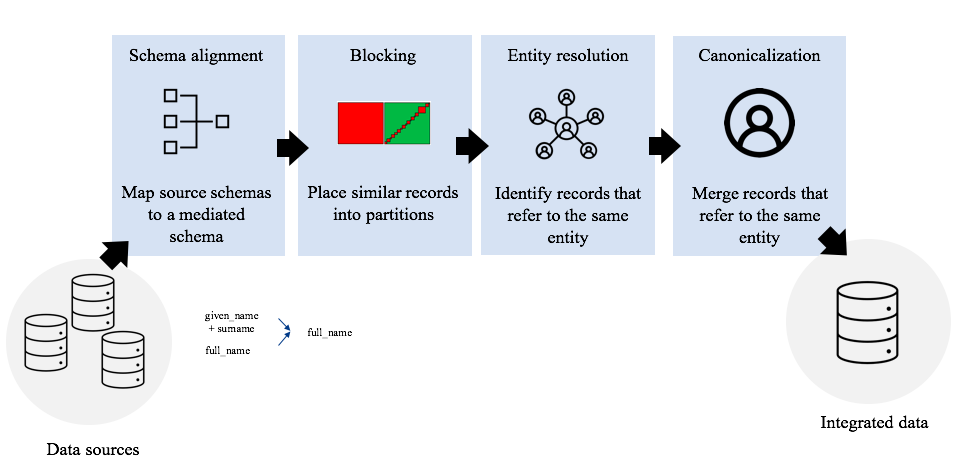
\includegraphics[scale=0.3]{finalFigures/pipeline}
%\caption{default}
\label{default}
\end{center}
\end{figure}

}


%\frame{
%\center
%\Large
%
%Entity resolution (record linkage or de-duplication) is the process of removing duplicated information from large noisy databases. 
%
%\pause
%
%\vspace*{1em}
%The purpose of this review is to introduce one to the fundamentals of entity resolution, its applications, and modern developments over the past 61+ years. 
%
%}

\frame{
\center
\Large

Let's consider a simple data cleaning application.

}

\frame{
\center


\begin{figure}[htbp]
\begin{center}
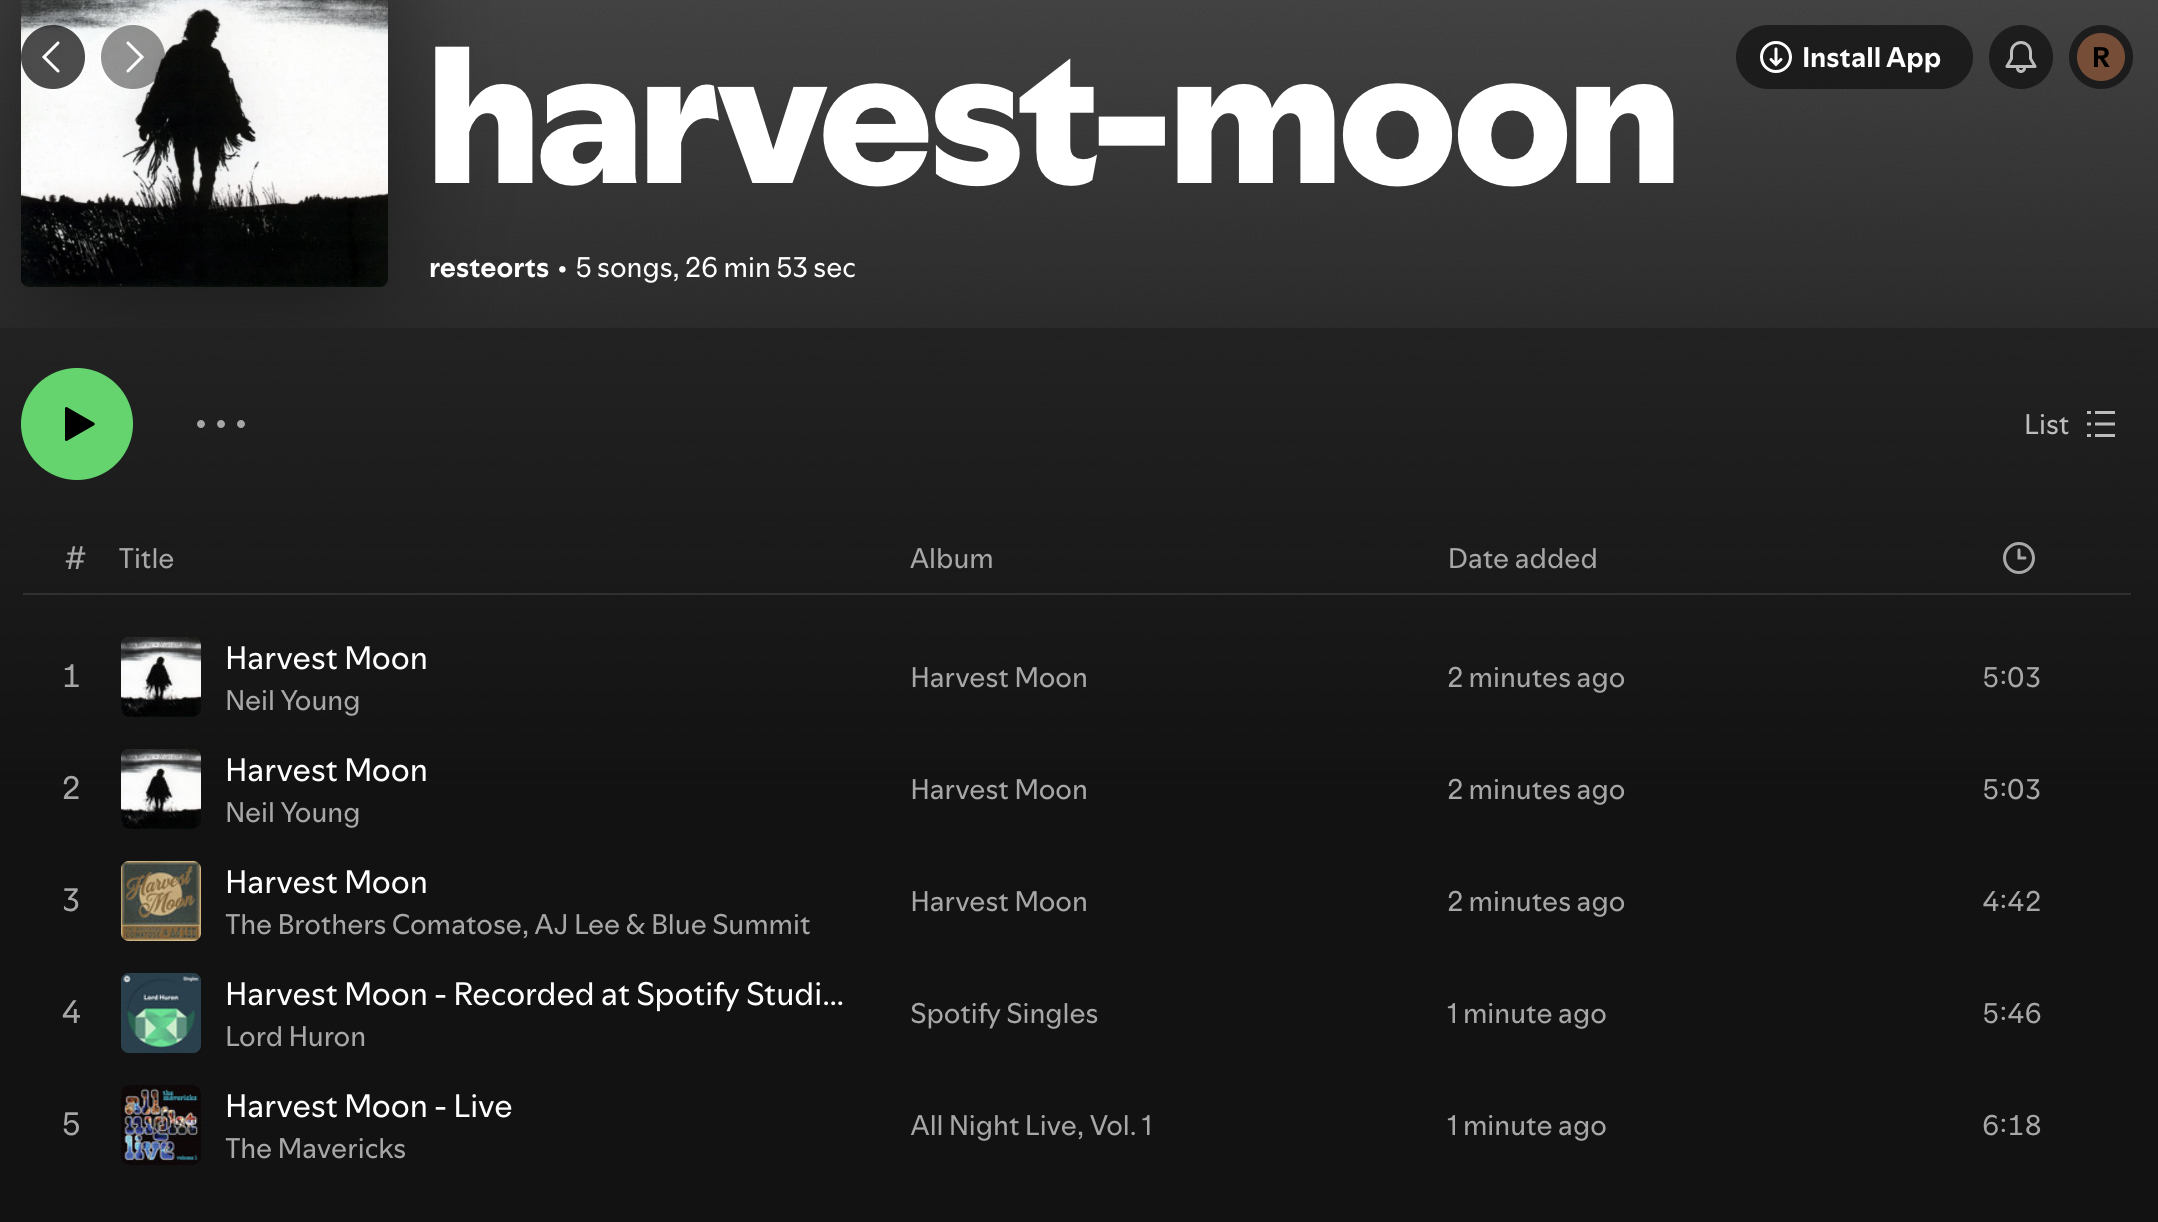
\includegraphics[width=\textwidth]{finalFigures/harvest-moon}
\caption{How many unique songs can you identify visually?}
\label{default}
\end{center}
\end{figure}

}

\frame{
\center


\begin{figure}[htbp]
\begin{center}
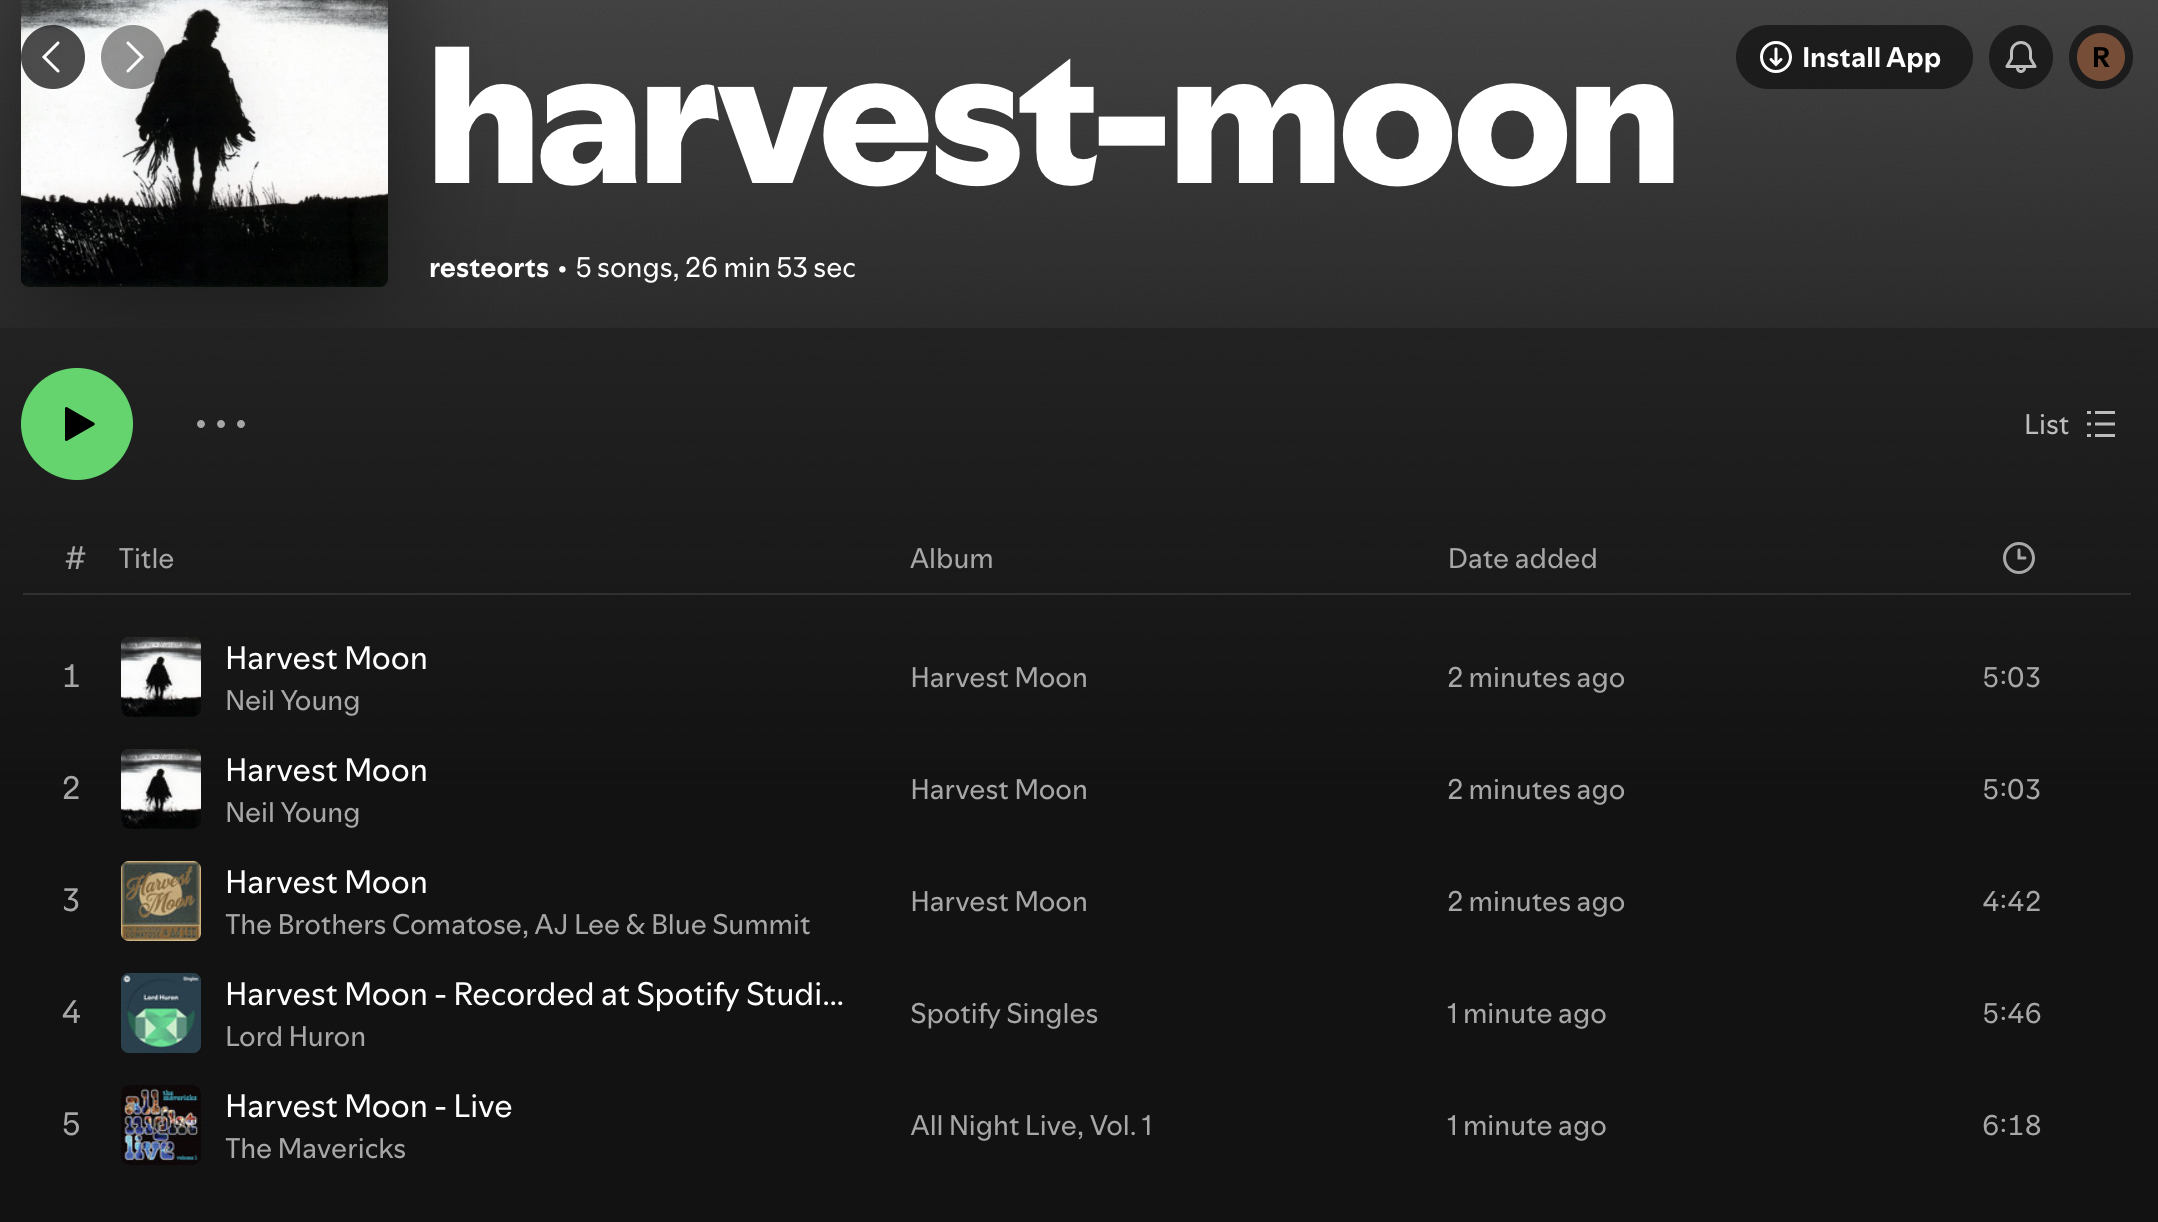
\includegraphics[width=\textwidth]{finalFigures/harvest-moon}
\caption{How could you automate this with millions of songs to have a clean, unique database of songs?}
\label{default}
\end{center}
\end{figure}

}



\frame{
\center
\Large

Let's consider a more challenging one!

}

\frame{
\frametitle{Human Rights Applications}

\begin{figure}[htbp]
\begin{center}
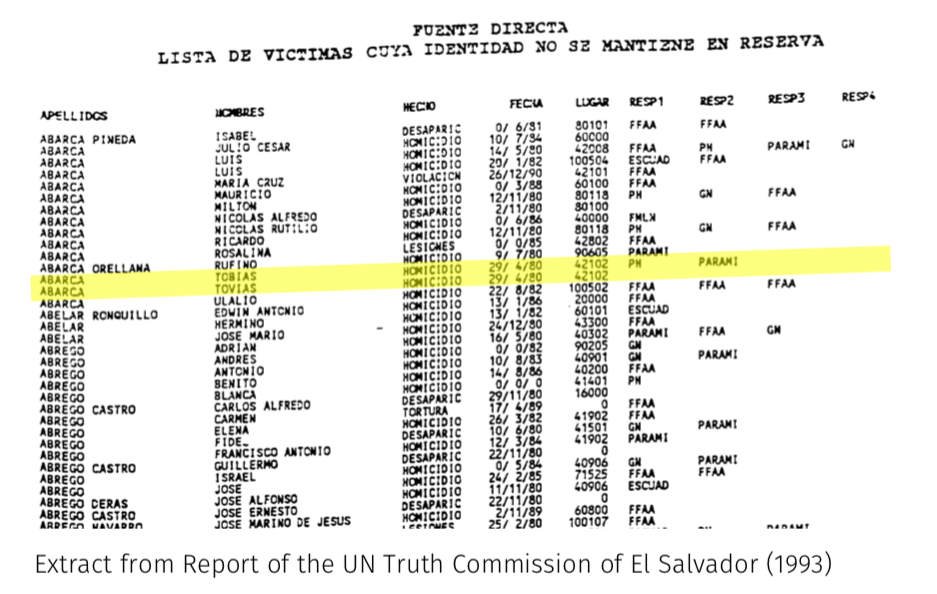
\includegraphics[scale=0.3]{finalFigures/untc.png}
\caption{Original Information from the El Salvadoran Conflict before data is cleaned.}
\label{default}
\end{center}
\end{figure}

}

\frame{
\frametitle{Human Rights Applications}

\begin{figure}[htbp]
\begin{center}
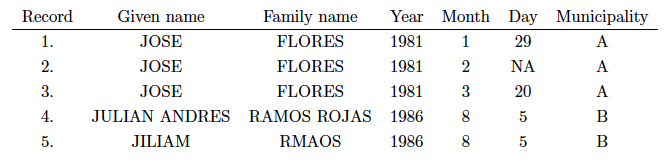
\includegraphics[scale=0.35]{finalFigures/untc-sadinle}
\caption{Snapshot from El Salvadoran Conflict. What seems difficult regarding this type of information?}
\label{default}
\end{center}
\end{figure}

}

\frame{
\frametitle{Voter Registration Applications}

\begin{figure}[htbp]
\begin{center}
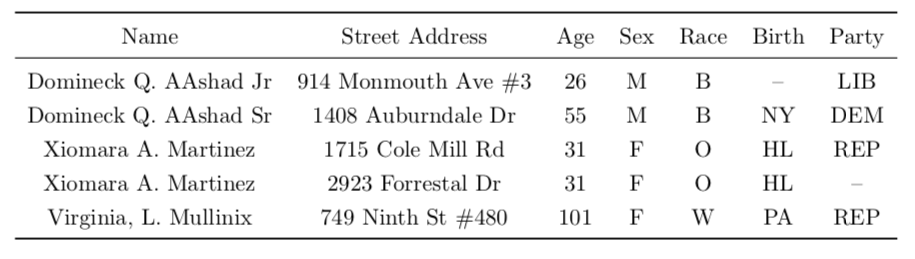
\includegraphics[scale=0.35]{finalFigures/voter}
\caption{Snapshot from the North Carolina Voter Registration Data Set}
\label{default}
\end{center}
\end{figure}

}


\frame{
\center

\begin{itemize}
\item Can you think of other applications where entity resolution would be needed or you have seen this before? 
\item Can you think of why the problem would be important?
\item Can you think of some challenges of this problem?
\item Why does this problem impact general machine learning, such as prediction and inference? 
\end{itemize}

}



\frame{

\center
\Large
Questions?\\
beka@stat.duke.edu\\
Webpage: \url{resteorts.github.io} \\ 
Software: \url{https://github.com/orgs/cleanzr/}\\
Paper: \url{https://arxiv.org/abs/2008.04443}


}

\clearpage
\newpage
\bibliographystyle{jasa}
\bibliography{er-review}




\end{document}